%==オプションおよび文書クラスの設定==
%"autodetect-engine"-どのエンジンでもコンパイル可能にするオプション
%"dvipdfmx-if-dvi"-必要な場合のみdvipdfmx経由のpdf化をするオプション(LuaTeXやXeTeXはPDFに直接変換するため)
%"ja=standard"-日本語文書の標準設定を利用するオプション
%"bxjs…"-どのエンジンでも利用可能なドキュメントクラス
%--以下のいずれかを選択--
\documentclass[autodetect-engine,dvipdfmx-if-dvi,ja=standard,a4paper,11pt]{bxjsarticle} %章の無いレポート
%\documentclass[autodetect-engine,dvipdfmx-if-dvi,ja=standard,a4paper,11pt]{bxjsslide} %スライド
%\documentclass[autodetect-engine,dvipdfmx-if-dvi,ja=standard,a4paper,11pt]{bxjsbook} %書籍
%\documentclass[autodetect-engine,dvipdfmx-if-dvi,ja=standard,a4paper,11pt]{bxjsreport} %章のある論文やレポート

%==プリアンブルの設定==
%--タイトル--
\title{順列エントロピーの説明} %タイトル
%\author{} %著者名
%\date{\today} %日付
%--パッケージの読込み及び設定の書換え--
\usepackage{multirow}
\usepackage{here} %図の挿入に関するパッケージ
\usepackage{ascmac} %枠に関するパッケージ
\usepackage{enumerate} 
\belowcaptionskip=-10pt %キャプション下の余白をN[pt]減らす
\usepackage{graphicx} %図の挿入に関するパッケージ
\usepackage{subcaption} %サブキャプションに関するパッケージ
\captionsetup{labelsep=space} %図名跡の":"を非表示にする
\usepackage{amsmath} %数式に関するパッケージ
\usepackage{mathtools} %数式に関するパッケージ
\usepackage{txfonts}  %数式に関するパッケージ
\usepackage{comment} %複数行のコメントアウトを可能にするパッケージ
\usepackage{bm} %ベクトル表示を可能にするパッケージ
\setpagelayout{top=10truemm,bottom=10truemm,left=10truemm,right=10truemm} %余白に関する設定の書換え(bxjs…クラスではgeometryパッケージは使用不可)
\graphicspath{{../figures/}} %図を挿入する際に.texファイルの上の階層にあるfiguresというフォルダを参照可能にする
\renewcommand{\labelitemi}{・}
\newcommand\longdiv[1]{\overline{\smash{)}#1}}
%==本文==
\begin{document}
\maketitle %設定したタイトルの挿入
%\tableofcontents
\section{順列エントロピー}
順列エントロピーとは,C.Bandt and  B. Pompe~\cite{PE2002}によって考案された,時系列の乱雑さを定量評価する指標であり,時系列の値そのものではなく,値の間の大小関係のみに注目し,時系列の特徴量を計算する手法である.
\par 時系列$ x(t) $を,$ D $次元の遅れ時間座標系$\bm{{\rm X}} _j=\left\{x_j, x_{j+\tau},...,x_{j+(D-1)\tau}\right\} $に埋め込む.ただし,$j=1,2,...,L-(D-1) \tau$とし,$L$は時系列の長さ,$D$は埋め込み次元,$\tau$は遅れ時間とする.
\begin{figure}[H]
\begin{center}
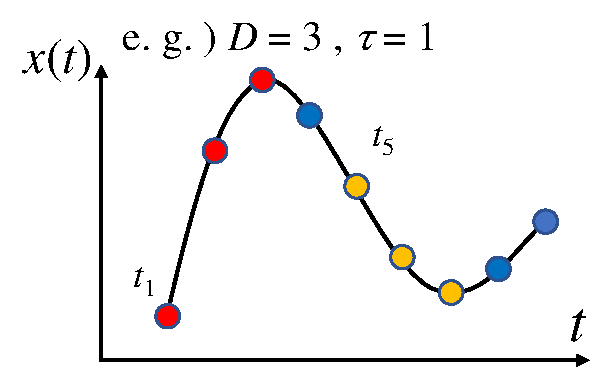
\includegraphics[width=.4\textwidth]{crop_PE1ver2.pdf} 
\end{center}
\caption{時系列$ x(t) $}%図名
\label{PE1}
\end{figure}
次元$ D $個分の点に着目し,それらの値の大小関係を比較する.ランクオーダーパターンは,$D!$個のいずれかのランクオーダーパターンに分類される.
\begin{figure}[H]
\begin{center}
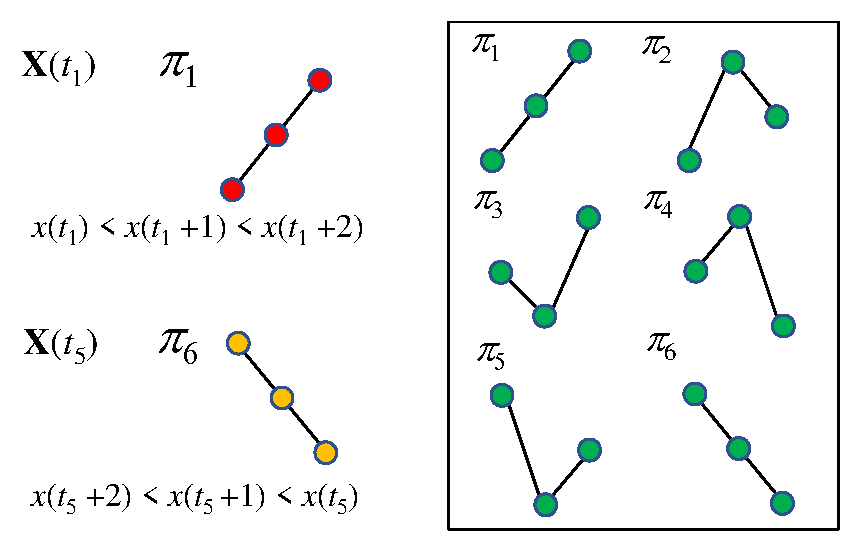
\includegraphics[width=.55\textwidth]{crop_PE2.pdf} 
\end{center}
\caption{ランクオーダーパターン}%図名
\label{PE21}
\end{figure}
あるランクオーダーパターン$\pi_i$の相対度数$p(\pi_i)$は,以下のように示される.
\begin{eqnarray}
p(\pi_i)=\dfrac{\sum_{j=1}^{N} \chi_{i}(X_{j})}{L-(D-1)\tau}
\end{eqnarray}
$\chi_{i}(X_{j})$は指示関数であり,以下のように示される.
\begin{eqnarray}
\chi_{i}(X_{j})=
\left\lbrace 
\begin{array}{l}
1, \rm{if} ~\pi_j=\pi_{i} \\
0, \rm{if} ~\pi_j \neq \pi_{i} 
\end{array}
\right.
\end{eqnarray}
\begin{figure}[H]
\begin{center}
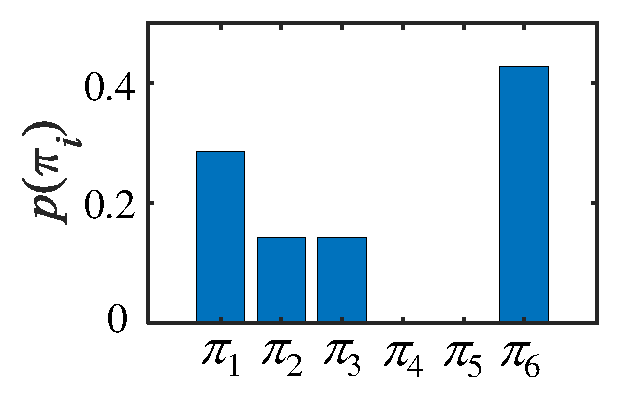
\includegraphics[width=.6\textwidth]{crop_PE3.pdf} 
\end{center}
\caption{ランクオーダーパターンの相対度数}%図名
\label{PE3}
\end{figure}
上で算出したランクオーダーパターン$\pi_i$の相対度数$p(\pi_i)$を情報エントロピーであるShannonエントロピーの式に代入することで,順列エントロピー$ H_p $は定義される.また,順列エントロピー$ H_p $が最大となるときは,すべてのランクオーダーパターンの相対度数が等確率で現れるときなので,$ H_{p,{\rm max}}=\log_2 D! $となる.
\begin{eqnarray}
H_p=\dfrac{-\displaystyle\sum_{i=1}^{D!} p(\pi_i) \log_2 p(\pi_i)}{\log_2 D!}
\end{eqnarray}
$H_p$が0に近いと時系列の周期性が高いことを示し,1に近ければ時系列の乱雑さが高いことを示す.



\begin{thebibliography}{9}
\bibitem{PE2002} C. Bandt and B.Pompe, "Permutation Entropy: A Natural Complexity Measure
for Time Series",~\textit{Physical Review Letters} \textbf{88}, 174102 (2002)
\end{thebibliography}

\end{document}